\section{Outlier detection/Anomaly detection}
We rank the observations using Gaussian Kernel density ( leave one-out), KNN density and KNN average relative density seperately. As shown in the following figures, the Gaussian Kernel density seems to be a good model for this data. ~\\

Gaussian Kernel density: From the figure we can find that the curve bends between 30\% to 40\%. Since the propotion of the spam emails in the data is 39.4\%. It seems that the Gaussian Kernel density can detect the spam emails as the outliers at a relative high accuracy.~\\

KNN density: The KNN density can only detect few outliers. It is impossible to find spam emails using this density.~\\

KNN average relative density: The KNN average relative density can detect some outliers. However, we cannot infer which part are the spam emails.

\begin{figure}[!ht]
	\centering
	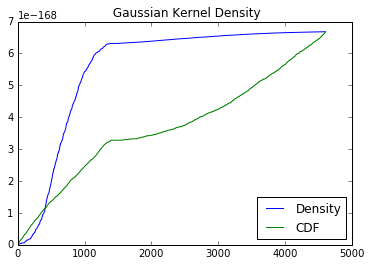
\includegraphics[width=0.5\textwidth]{Fig/gaussian.png}
	\vspace{-5pt}
	\caption{Gaussian Kernel density: Outlier score}
\end{figure}

\begin{figure}[!ht]
	\centering
	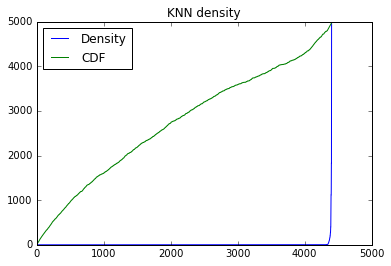
\includegraphics[width=0.5\textwidth]{Fig/knn.png}
	\vspace{-5pt}
	\caption{KNN density: Outlier score}
\end{figure}

\begin{figure}[!ht]
	\centering
	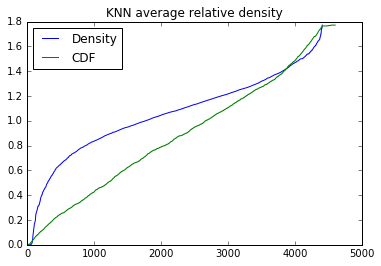
\includegraphics[width=0.5\textwidth]{Fig/knn_average.png}
	\vspace{-5pt}
	\caption{KNN average relative density: Outlier score}
\end{figure}
